\documentclass[12pt,a4paper]{article}
\usepackage[margin=.5in]{geometry}
\usepackage[utf8]{inputenc}
\usepackage[IL2]{fontenc}
\usepackage[czech]{babel}
\usepackage{microtype}
\usepackage{amssymb}
\usepackage{amsthm}
\usepackage{amsmath}
\usepackage{xcolor}
\usepackage{graphicx}

\usepackage[inline]{enumitem}

\newcommand{\R}{\mathbb{R}}

\DeclareMathOperator{\tg}{tg}
\DeclareMathOperator{\cotg}{cotg}

\setlist[enumerate]{label={(\alph*)},topsep=\smallskipamount,itemsep=\smallskipamount,parsep=0pt}
\setlist[itemize]{topsep=\smallskipamount,noitemsep}

\def\tisk{%
\newbox\shipouthackbox
\pdfpagewidth=2\pdfpagewidth
\let\oldshipout=\shipout
\def\shipout{\afterassignment\zdvojtmp \setbox\shipouthackbox=}%
\def\zdvojtmp{\aftergroup\zdvoj}%
\def\zdvoj{%
    \oldshipout\vbox{\hbox{%
        \copy\shipouthackbox
        \hskip\dimexpr .5\pdfpagewidth-\wd\shipouthackbox\relax
        \box\shipouthackbox
    }}%
}}%


\newtheorem*{poz}{Pozorování}

\theoremstyle{definition}
\newtheorem{uloha}{Úloha}
\newtheorem{suloha}[uloha]{\llap{$\star$ }Úloha}
\newtheorem*{bonus}{Bonus}
\newtheorem*{defn}{Definice}

\pagestyle{empty}

\let\ee\expandafter

\def\vysld{}
\let\printvysl\relax
\let\printalphvysl\relax

\makeatletter
\long\def\vyslplain#1{\ee\ee\ee\gdef\ee\ee\ee\vysld\ee\ee\ee{\ee\vysld\ee\printvysl\ee{\the\c@uloha}{#1}}}
\let\vysl\vyslplain

\def\locvysl#1{\ee\gdef\ee\locvysld\ee{\locvysld\item #1}}
\let\lv\locvysl

\newenvironment{ulohav}[1][]{\begin{uloha}[#1]\gdef\locvysld{\begin{enumerate}}}{\ee\vyslplain\ee{\locvysld\end{enumerate}}\end{uloha}}
\newenvironment{sulohav}[1][]{\begin{suloha}[#1]\gdef\locvysld{\begin{enumerate*}}}{\ee\vyslplain\ee{\locvysld\end{enumerate*}}\end{suloha}}

\makeatother

\begin{document}

%\tisk

\section*{Dělitelná všehochuť}
% vykradacka starych Naboju / PraSete

\begin{uloha}
Do každého kolečka napište jedno z čísel $2$, $3$, $4$, $5$, $6$, $11$, $13$, $21$, $30$, $34$ a $6006$ tak, aby poměr čísel ve dvou kolečkách byl celočíselný právě tehdy, když jsou tato kolečka spojená čárou.
\[ 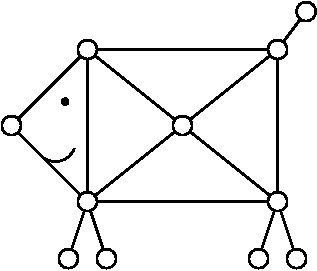
\includegraphics{prase.pdf} \]
\end{uloha}


\begin{uloha}
Nalezněte nejmenší přirozené číslo, které končí na $17$, je dělitelné $17$ a má ciferný součet $17$.
\vysl{15317}
\end{uloha}


\begin{uloha}
$a679b$ je pěticiferné číslo dělitelné $72$. Zjistěte hodnotu součinu $a \cdot b$.
\vysl{6}
\end{uloha}


\begin{uloha}
Míša objevila šesticiferné přirozené číslo splňující následující podmínky: 
\begin{itemize}
\item Číslo se čte stejně zleva doprava i zprava doleva. 
\item Je dělitelné devíti.
\item Po škrtnutí první a poslední cifry je jediným prvočíselným dělitelem nového čísla číslo 11. 
\end{itemize}
Které číslo Míša objevila?
\vysl{513315}
\end{uloha}


\begin{uloha} % vyzaduje kombinatorickou uvahu
Kolik je trojciferných čísel dělitelných šesti takových, že v~nich je každá cifra větší než $4$?
\vysl{16}
\end{uloha}


\begin{uloha}
Martin si napsal své oblíbené číslo do sešitu. Petr mu ho vzal a škrtl cifru na místě jednotek. Pak si všiml, že původní číslo je dělitelné tím novým. Najděte všechna dvouciferná čísla, která mohl Martin napsat.
\vysl{10, 11, 12, 13, 14, 15, 16, 17, 18, 19, 20, 22, 24, 26, 28, 30, 33, 36, 39, 40, 44, 48, 50, 55, 60, 66, 70, 77, 80, 88, 90, 99}
\end{uloha}


\begin{uloha}
Dva rozmazlení bratříčci Viktor a Mišo dostali pytel bonbonů, který si půl na půl rozdělili. Každý z nich sní během dne dva až tři bonbony. Malému Vikouškovi bonbony vydržely na čtrnáct dní, staršímu Mišovi přesně na tři týdny. Kolik bonbonů bylo původně v pytli?
\vysl{84}
\end{uloha}


\begin{uloha}
Alčino oblíbené číslo má následující vlastnosti:
\begin{itemize}
\item Má celkem osm cifer.
\item Jeho cifry jsou navzájem různé a zleva doprava se zmenšují.
\item Je dělitelné 180.
\end{itemize}
Jaké je to číslo?
\vysl{97654320}
\end{uloha}


\begin{uloha}
Štěpán dal Lukášovi hádanku. Vybral si číslici $X$ a řekl: "`Myslím si trojciferné číslo dělitelné jedenácti. Na pozici stovek má číslici $X$ a na pozici desítek trojku. Tvým úkolem je zjistit číslici na pozici jednotek."' Lukáš se na chvilku a zamyslel a vykřikl: \uv{Ha, už vím, jak na to!} Ale pak si uvědomil, že hádanka nemá řešení -- žádná číslice na pozici jednotek nevyhovuje popsaným vlastnostem Štěpánova čísla. Jakou číslici Štěpán za $X$ vybral?
\vysl{4}
\end{uloha}


\begin{uloha}
Jednoho dne potkal nebojácný Oidipus Sfingu, která mu položila hádanku. Vymyslela si dvojciferné číslo $S$ a následně umožnila Oidipovi vybrat tři různá jednociferná čísla $a<b<c$ a pro každé z~nich se zeptat, zda je jím $S$ dělitelné. Poté, co Oidipus obdržel tři odpovědi ano/ne, měl číslo $S$ uhádnout. Upadl však do zoufalství, neboť tyto podmínky splňovala právě dvě různá čísla. Naštěstí mu Sfinga krátce nato sdělila, že se spletla v~dělitelnosti $b$, což mu umožnilo číslo $S$ s~jistotou určit. Jaké bylo číslo $S$?
\vysl{84}
\end{uloha}


\newpage
\parindent=0pt
\parskip=\smallskipamount
\def\printvysl#1#2{\textbf{#1.}\ #2\par}
\vysld


\end{document}